% =====================================================================
% Voxplay -- IEEE conference paper, Overleaf-ready.
%
% Overleaf: create a Blank Project, paste this in as main.tex, and upload
%   figures/fig1-pipeline.png
%   figures/fig2-pacing.png
% IEEEtran is already installed on Overleaf; nothing else is needed.
% Compile with pdfLaTeX.
%
% TO FILL IN: the \author block below. Everything else is final.
% =====================================================================
\documentclass[conference]{IEEEtran}
\IEEEoverridecommandlockouts

\usepackage{cite}
\usepackage{amsmath,amssymb}
\usepackage{graphicx}
\usepackage{booktabs}
\usepackage{url}
\usepackage[T1]{fontenc}
\usepackage[utf8]{inputenc}

\graphicspath{{figures/}}

% Tighter tables; IEEE columns are narrow.
\newcommand{\tabsize}{\footnotesize}

\begin{document}

\title{Voxplay: Pacing and Verifiable Grounding for Spoken\\
Chess Commentary Generated from Move Notation}

\author{%
\IEEEauthorblockN{First Author, Second Author, Third Author, Fourth Author}
\IEEEauthorblockA{\textit{Department, Institution}\\
Guide: Guide Name, Designation\\
City, Country\\
email@institution.edu}
}

\maketitle

\begin{abstract}
Millions of chess games are played online daily and almost none are
explained. Engine analysis yields a table of labels; human commentary exists
only for elite play. Prior work emits one comment per move as text and
measures factual accuracy after generation rather than constraining it.
Voxplay turns move notation alone into spoken commentary synchronised to an
animated board. First, commentary is \emph{paced}: beat selection is
budgeted maximum-weight selection, solved greedily to a mean 98.7\% of the
exact optimum. Over 173 standard Lichess games it runs 3.6$\times$ shorter
than move-by-move narration while covering the opening and finish in every
one. Second, the model is never asked to derive a chess fact; facts come
from deterministic components validated externally --- 91.9\% mean recall
and 89.9\% precision over 14,000 human-tagged puzzles, and $\kappa = 0.955$
for the classification rule against Lichess annotations on a held-out 6,864
moves, falling to 0.673 once our own engine supplies the evaluations. Third,
every sentence is checked against the facts licensing it, and the check is
itself auditable: run over grounded text it exposed a licence defect we then
fixed, leaving 0.66 false positives per 100 beats, though the checks are
lexical and cannot see a sentence that misuses licensed vocabulary.
Generation costs US\$0.06 per game.
\end{abstract}

\begin{IEEEkeywords}
sports commentary, data-to-text generation, content selection, grounded
generation, hallucination mitigation, chess
\end{IEEEkeywords}

% =====================================================================
\section{Introduction}

A chess game is a complete and unambiguous record: every move is known,
every position computable, and a strong engine can quantify the consequence
of each decision. Yet what an ordinary player gets afterwards is a table ---
moves tagged \emph{blunder}, \emph{mistake} or \emph{inaccuracy} beside
numeric evaluations. It says a move was bad, not what was missed, which of
eighty moves decided the game, or why; and it cannot be listened to. Human
commentary supplies all of that and is restricted to elite play. This paper
describes a system occupying that gap: the input is the move list, and the
output is spoken audio with a board that follows the narration, with no
video and no vision model involved.

Chess admits this because its facts are computable and checkable. That
permits a pipeline in which the model is never asked to derive a chess fact
and every sentence it writes is checked against the facts it was given.
Neither step makes invention impossible --- the ungated pilot of Section
\ref{sec:gate-results} produced two unsupported claims in 32 beats --- but
together they remove the occasion for it and give a mechanical test for what
survives. The same property is why the approach generalises less readily to
domains whose ground truth must itself be inferred.

\textbf{Contributions.}
(i) \emph{Pacing as budgeted selection}: we formalise what to say as
maximum-weight selection under a spoken-duration budget and minimum
separation, give the objective and constraints explicitly, name the solver
and bound its suboptimality against an exact dynamic program, with two
baselines implemented in the same codebase.
(ii) \emph{Grounding by construction}: all chess facts are computed by
independently validated deterministic components and supplied as a closed
fact block.
(iii) \emph{A verification gate with a symmetric licence} derived from the
same function that builds those facts, whose false-positive rate we measure
rather than assume.
(iv) \emph{Speech with a measured timeline}, offsets coming from the
rendered waveform rather than word counts.

% =====================================================================
\section{Related Work}

\textbf{Chess commentary.} Jhamtani et al. \cite{jhamtani2018} introduced
the task from forum discussion; Zang et al. \cite{zang2019} coupled
generation to a neural engine; Lee et al. \cite{lee2022} added symbolic
reasoning; Kim et al. \cite{kim2025} introduced concept-guided generation
with a dedicated metric. All four generate text per move. Concept
prioritisation \cite{kim2025} selects what to say \emph{about a move}; none
selects which moves to speak about at all, which is what a listener
experiences as pacing.

\textbf{Factuality.} Hebbar et al. \cite{hebbar2026} report GPT-5.4
producing incorrect sub-claims 22.0\% of the time without tools, open-weight
models exceeding 40\%; their contribution is evaluation \emph{after}
generation. Ji et al. \cite{ji2023} distinguish intrinsic from extrinsic
hallucination; we target the extrinsic kind by making the admissible fact
set finite and explicit.

\textbf{Content selection.} Barzilay and Lapata \cite{barzilay2005} framed
content selection as a constrained decision over candidate records; Wiseman
et al. \cite{wiseman2017} showed on RotoWire that fluent generation from
structured records implies neither faithful nor well-selected content;
Puduppully et al. \cite{puduppully2019} made selection and ordering explicit
as a content plan. Our formulation adds a \emph{duration} budget, meaningful
only once output is spoken.

\textbf{Other sports.} MatchTime \cite{rao2024} and SoccerNet-Caption
\cite{mkhallati2023} generate soccer commentary from video, where ground
truth is inferred rather than computed; a survey \cite{zheng2026} confirms
the pattern. That a language model can write chess commentary is
established; our claims are pacing, spoken delivery and grounding enforced
by construction.

% =====================================================================
\section{System Architecture}

The pipeline has six stages (Fig.~\ref{fig:pipeline}): ingest notation into
move events; evaluate every position; detect motifs and opening deviation;
select and pace beats; realise the facts as prose; and verify, then speak.

\begin{figure}[!t]
\centering
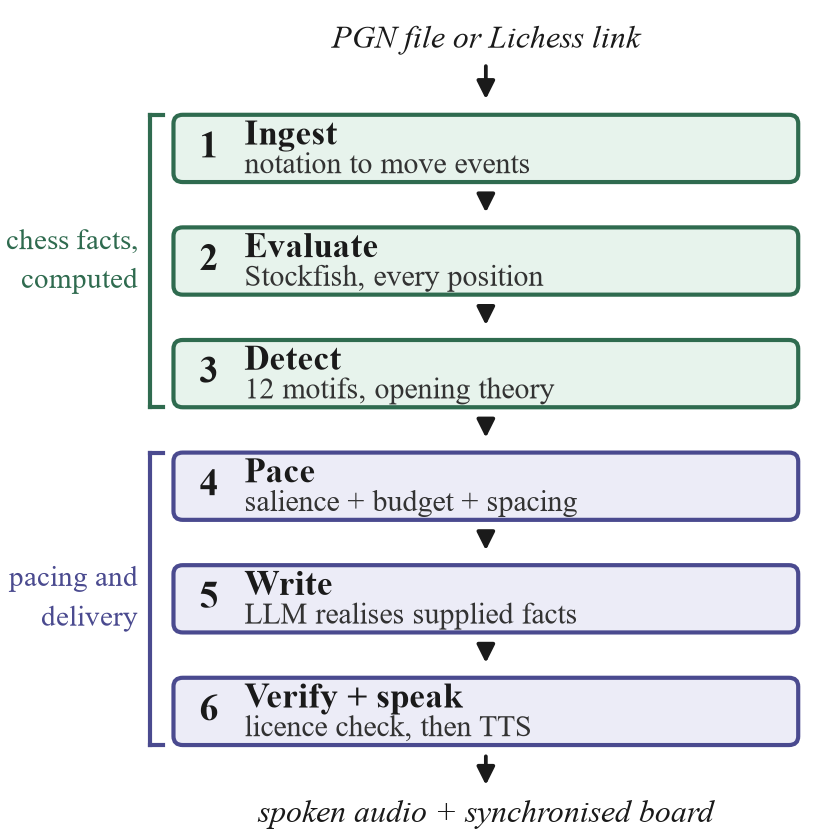
\includegraphics[width=0.78\columnwidth]{fig1-pipeline.png}
\caption{The six-stage pipeline. Stages 1--3 compute chess facts before the
model is invoked; stages 4--6 pace, realise and speak them.}
\label{fig:pipeline}
\end{figure}

The architectural invariant is the boundary between fact computation and
generation: everything the narration may assert is computed before the model
is invoked, and the dependency graph is acyclic, so beat selection can be
tested without an engine and verification without an API key. The
implementation is roughly 11,600 lines of Python with 555 automated tests,
using python-chess, Stockfish and \texttt{claude-opus-5}.

% =====================================================================
\section{Method}

\subsection{Evaluation in win probability}

Centipawn differences are not comparable across positions: losing 100
centipawns from $+900$ is irrelevant, whereas losing 100 from equality can
decide the game. Every evaluation is therefore mapped to win probability by
the logistic published by Lichess \cite{lichessaccuracy}, with centipawns
$c$ clamped to $\pm 1000$ and $\lambda = 0.00368208$:

\begin{equation}
W(c) = 50 + 50\left(\frac{2}{1 + e^{-\lambda c}} - 1\right)
\end{equation}

The mapping saturates at the extremes, so the same 100-centipawn delta is
worth 9.1 points of win probability from equality but 1.5 from $+800$ --- a
six-fold difference, which is the property centipawns lack. Every downstream
component reads $W$, and the constant is adopted from Lichess so our
classifications are directly comparable with Lichess's own annotations.
Analysis is budgeted by \textbf{nodes}, not depth or wall-clock time, since
time-limited search returns different results on different machines and
would make every number here irreproducible: 1,000,000 nodes per position,
\texttt{MultiPV} 3 and a \textbf{single search thread} (Section
\ref{sec:limitations}).

\subsection{Move classification}
\label{sec:classification}

Let $L$ be the win probability the mover lost. A move is \texttt{best} if it
is the engine's top choice, \texttt{book} if also within opening theory,
otherwise \texttt{good}, \texttt{inaccuracy}, \texttt{mistake} or
\texttt{blunder} as $L$ falls below 5, in $[5,10)$, in $[10,15)$, or at or
above 15. A commentary variant caps severity at \texttt{inaccuracy} once the
mover's $W$ exceeds 90, since calling a move a blunder while the player is
still completely winning misdescribes the position; the cap is disabled for
Section \ref{sec:agreement}.

Community documentation gives the bands as roughly 10/20/30, about twice too
lenient. Fitting $\theta$ to maximise agreement recovers 5/10/15 --- exactly
Lichess's documented 0.1/0.2/0.3 winning-chances delta rescaled to 0--100
--- so our claim is correspondingly modest: a high $\kappa$ shows the
implementation is \textbf{faithful}, not that a new method has been found.

\subsection{Motifs and opening theory}

Twelve motifs are detected from board geometry alone, with no engine and no
language model: fork, pin, skewer, discovered attack, hanging piece,
sacrifice, back-rank mate, smothered mate, double check, promotion, en
passant and advanced pawn. A model asked whether a position contains a fork
answers confidently either way, and a listener who plays chess catches the
error. Detector names match Lichess puzzle themes, so validation is a direct
comparison. Geometry shows material was given up but not that a sacrifice
was \emph{sound}; soundness is decided in the analysis layer. Naming the
opening by prefix-matching moves would miss every transposition, so we
instead replay each line of the CC0 \texttt{lichess-org/chess-openings}
database and index the resulting \textbf{position}.

\subsection{Pacing as budgeted selection}
\label{sec:pacing}

For each half-move $m$ of a game $M$ we compute six normalised signals in
$[0,1]$ --- evaluation swing $s$, narrative role $n$, strongest motif $t$,
criticality $k$ (the gap between best and second-best move), material swing
$a$, and think time $h$ relative to that player's own baseline --- combined
with weights $\mathbf{w} = (1.00, 0.60, 0.45, 0.35, 0.25, 0.20)$:

\begin{equation}
\sigma(m) = w_s s + w_n n + w_t t + w_k k + w_a a + w_h h
\end{equation}

Swing saturates at the blunder threshold, so any blunder maxes that term.
Each beat costs $c(m)$ spoken \textbf{words}, fixed by type: 65 for the
turning point, 45 for an ordinary moment. Writing $x_m \in \{0,1\}$ for the
decision to speak about $m$, and $P \subseteq M$ for candidates clearing a
floor $\sigma(m) \geq 0.25$ and not already covered by a mandatory beat,
selection solves:

\begin{align}
&\text{maximise} && \sum_{m \in P} \sigma(m)\, x_m \\
&\text{subject to} && \sum_{m \in P} c(m)\, x_m \leq B \\
&&& x_i + x_j \leq 1 \;\;\text{if}\;\; |\mathrm{ply}(i) - \mathrm{ply}(j)| < g
\end{align}

\noindent with separation $g = 4$ half-moves. A listener's budget is a
duration but the selector adds up words, related by the measured rate
$r = 1.85$ words per second. The target duration $T$ scales with game
length, clamped at both ends, and $B$ is that duration in words less those
already committed to the mandatory intro, opening, finish and outro beats
$R$, which supply the coverage requirement directly rather than as a
constraint:

\begin{equation}
T(M) = \min\bigl(360, \max(150,\, 2|M|)\bigr) \;\text{seconds}
\end{equation}

\begin{equation}
B = \left\lfloor r \cdot T(M) \right\rfloor - \sum_{j \in R} c(j)
\end{equation}

For a 33-half-move game $T = 150$\,s, so $r \cdot T = 277$ words; the
mandatory beats cost 153, leaving $B = 124$ --- a turning point and one
further moment. A fixed budget does not transfer across game lengths.

\textbf{Solver and optimality.} Equations (3)--(5) are solved
\textbf{greedily}: candidates sorted by $\sigma$ descending are accepted if
they fit the budget and violate no separation constraint, which is
$O(|M| \log |M|)$ in practice. Greedy is not optimal in general, but the
problem is exactly solvable: with candidates in ply order, (5) between
\emph{consecutive} chosen candidates implies it for every pair, so (3)--(5)
is a knapsack on a line admitting an exact $O(|P| \cdot B)$ dynamic program,
tractable because $c$ is integral in words. We implement it as a reference
and report the gap in Section \ref{sec:optimality}. Finally, $r = 1.85$ is
measured, not nominal: a 134-word script rendered at a nominal 155 wpm
produced 72.6\,s of audio, an effective 111 wpm.

\subsection{Script generation}

One call establishes a through-line; each beat is then realised in a
separate call receiving the outline, the lines already spoken, and a
\textbf{fact block} that is the complete and only basis for that sentence.
Notation is converted to spoken form by rule, not by prompt: asking a model
to read ``Qxh7\#'' aloud succeeds most of the time and then produces ``queen
x h seven hash'' on the move that matters. For full-coverage sheets, beats
are generated in runs of six and parsed back by index, the batch rejected
entirely if the shape is wrong --- a partially parsed batch would attach one
move's commentary to another, an error in which every individual claim stays
true and which the verifier therefore cannot detect.

Four prompts are sent beneath one cached system prompt --- outline, per-beat
realisation, a batched variant, and a repair prompt appending the verifier's
finding --- all verbatim in supplementary Section S1. The system prompt
states that every chess fact must appear in the FACTS block, notation must
never be written, and no numeric evaluation may be stated. The architecture
does not rely on the model obeying these: the fact block is the only chess
content in the context, and the output is checked against a licence built by
the same function.

\subsection{The verification gate}
\label{sec:gate}

Each sentence is checked against a \textbf{licence}: the claims the beat's
facts support --- permitted squares, motifs, names, the evaluation, and
whether the result may be revealed. Seven checks run: notation leakage,
ungrounded squares, ungrounded tactics, evaluation contradiction, ungrounded
names, cross-beat repetition and length. The first five are factual defects;
the last two are stylistic warnings, excluded from every error rate below.

The licence is derived from the same function that builds the fact block.
This symmetry matters in both directions: a fact supplied but not licensed
produces a false positive, and a claim licensed but never supplied produces
a blind spot. Section \ref{sec:gate-results} measures the first and finds
one. A failing beat is \textbf{regenerated} with the failure fed back, and
the same gate checks text a user edited by hand, so an invented claim typed
by a person is caught identically.

\textbf{What the licence cannot express.} Every check is lexical: which
squares, motif names, player names and evaluation direction appear. A
sentence drawing only on licensed vocabulary can therefore be false about
the position and pass. Five such sentences, each built from one beat's own
licence, pass all seven checks: giving the move to the wrong side, naming a
licensed square but the wrong piece on it, attaching a licensed motif to a
move that did not create it, a strategic claim with no lexical anchor
(``controls the centre''), and revealing the outcome without a result word.
Two controls reaching outside the licence are caught, so the checks fire
when they can. The gate bounds what may be \emph{named}, not what may be
\emph{asserted} about it.

\subsection{Speech and timeline}

Audio offsets are measured from the rendered waveform, never estimated, and
compressed clips are transcoded before any offset is taken, so the choice of
voice cannot silently desynchronise the board. Each clip is synthesised with
its neighbouring lines as unspoken context \cite{xu2021}; without it a line
closes as though the game ended there, and a six-beat recap is heard as six
announcements rather than one person speaking.

% =====================================================================
\section{Experimental Validation}

All results are measured against externally produced labels this project did
not generate. Every number is produced by a script in
\texttt{docs/paper/studies/}; supplementary Section S4 maps scripts to
tables.

\textbf{Corpus and inclusion criterion.} The corpus is a PGN export of
analysed Lichess games (CC0), seeded from Lichess TV --- which carries the
variant channels, so the raw export of 339 games proved to be \textbf{174
standard and 165 variant games}. Every result below uses the standard subset
only: Stockfish declines Antichess outright; for Horde, Atomic, King of the
Hill, Racing Kings and Three-check the win condition differs, so a standard
engine's evaluation does not mean what (1) assumes; and although Chess960
shares the rules, the engine wrapper does not set \texttt{UCI\_Chess960}. An
earlier version of this work applied no such criterion and reported 14 games
lost to ``engine failures'' that were in fact Stockfish refusing Antichess,
leaving a corpus roughly half variants scored by a standard engine.

\subsection{Motif detection: precision and recall}

For each detector, 1,000 puzzles carrying its own theme were drawn by
reservoir sampling over 6.5 million rows of the Lichess puzzle database
(CC0) \cite{lichessdb}, with 2,000 controls from five non-motif themes ---
14,000 puzzles in all. A detector is credited if it fires anywhere among the
solver's moves, since a Lichess theme describes the whole solution, not its
first move. Across the eleven comparable detectors the mean is
\textbf{91.9\% recall and 89.9\% precision}, F1 0.904; three reach 1.000 and
the per-detector table is in supplementary Section S7.

Precision is reported at this 1,000-to-2,000 sampling ratio, not the
prevalence of motifs in commentary, and is a \textbf{lower bound} because
Lichess tags are not exhaustive. That is measurable: the back-rank detector
fired on 232 controls and replaying each line shows \emph{all 232 do finish
in checkmate on a back rank}, so its 81.2\% is an artefact of tagging.
Hanging piece is excluded because Lichess tags it when the solution
\emph{takes} an undefended piece whereas we detect a move that \emph{leaves}
one hanging. The pin detector is the one genuine weakness, trading recall
for precision at 49.2\% against 63.5\% unfiltered.

\subsection{Classification agreement, fitted and tested on disjoint splits}
\label{sec:agreement}

Lichess publishes both halves of what this needs: \texttt{[\%eval]} on every
move and its own verdict as a NAG. This section uses all 174 standard games,
counting only the 13,230 half-moves that carry an evaluation --- a game's
unannotated tail cannot be scored, so it is not counted. Games --- not moves
--- were shuffled under a fixed seed and split in half; $\theta$ was
grid-searched on the training half alone, and $\kappa$ reported on the
other.

\begin{table}[!t]
\caption{Agreement with Lichess labels, fitted and tested on disjoint splits}
\label{tab:agreement}
\centering
\tabsize
\begin{tabular}{lcc}
\toprule
 & \textbf{Train, 87} & \textbf{Held out, 87} \\
\midrule
Moves & 6,366 & 6,864 \\
$\theta$ fitted on train & 5 / 10 / 15 & --- \\
$\kappa$, our rule on Lichess evals & 0.957 & 0.955 \\
$\kappa$, documented 10/20/30 & --- & 0.343 \\
$\boldsymbol{\kappa}$\textbf{, our engine's evals} & --- & \textbf{0.673} \\
Raw agreement, our engine & --- & 90.8\% \\
Expected by chance & --- & 71.9\% \\
\bottomrule
\end{tabular}
\end{table}

Held-out $\kappa$ is within 0.002 of training $\kappa$, so there is no
measurable overfitting --- unsurprising, since the search recovers a
published constant rather than discovering a free parameter.

That figure is close to tautological, though, and the last two rows matter
more. $\kappa = 0.955$ has both sides reading \emph{Lichess's} evaluations,
so it isolates the rule and says little beyond that our implementation of a
formula adopted from Lichess is faithful. The shipped pipeline does not read
those evaluations: it runs Stockfish at 1,000,000 nodes on one thread.
Scoring the same held-out games from \textbf{our} engine against the same
labels gives $\boldsymbol{\kappa = 0.673}$, raw agreement 90.8\%, per-class
53.2\%, 41.3\% and 84.1\%. That 0.282 difference is two engines at two
search efforts disagreeing about borderline moves, and the rule-only figure
hides all of it.

Neither number is accuracy --- Lichess's annotations are another engine's
output, not ground truth --- so this measures agreement between two
configurations. The rule is faithful; the pipeline is substantially rather
than almost perfectly aligned with a reference system; and the circulated
10/20/30 bands are about twice too lenient, yielding $\kappa = 0.343$.

\subsection{Pacing over 173 games}
\label{sec:pacing-results}

The selector was run over the 173 standard games of 20--200 half-moves, one
game of the 174 being too short. Pacing needs every half-move, annotated or
not, so this section counts all 13,251 of them rather than the 13,230
evaluated ones of Section \ref{sec:agreement}; median length is 68 (IQR
55--92). No run failed.

\begin{table}[!t]
\caption{Pacing against both baselines over 173 standard games}
\label{tab:pacing}
\centering
\tabsize
\begin{tabular}{lccc}
\toprule
 & \textbf{Paced} & \textbf{Top-$N$} & \textbf{Every move} \\
\midrule
Median duration & \textbf{143.2\,s} & 194.6\,s & 514.6\,s \\
IQR & 142.2--178.4 & constant & 416.2--696.2 \\
Range & 117.8--348.6 & 194.6 & 158.9--1483.2 \\
Median beats & 7 & 8 & --- \\
Opening covered & \textbf{100\%} & 22.5\% & 100\% \\
Decisive move covered$^{*}$ & 98.8\% & 100\% & 100\% \\
Finish covered & \textbf{100\%} & 7.5\% & 100\% \\
No adjacent pick & \textbf{173/173} & 1/173 & --- \\
\bottomrule
\end{tabular}

\vspace{2pt}
\raggedright\footnotesize $^{*}$Over the 170 games that have a decisive
move; three drawn games have none.
\end{table}

\begin{figure}[!t]
\centering
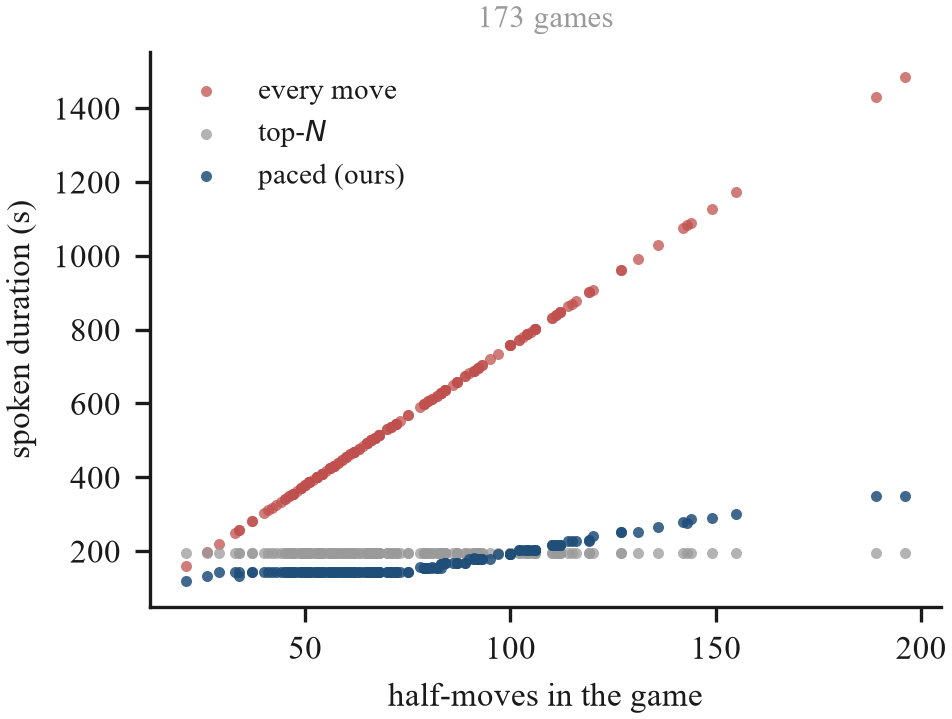
\includegraphics[width=0.84\columnwidth]{fig2-pacing.png}
\caption{Spoken duration against game length over 173 standard games. The
paced arm is clamped by (6); the every-move baseline grows without bound;
top-$N$ is constant by construction.}
\label{fig:pacing}
\end{figure}

Median reduction against every-move narration is \textbf{3.6$\times$} (IQR
2.9--3.9), widening with game length because the paced budget is clamped by
(6) and the baseline's is not (Fig.~\ref{fig:pacing}). Top-$N$ emits exactly
$N = 8$ beats of fixed cost, so its 194.6\,s is \textbf{constant by
construction} --- worth stating, since an identical figure across games
otherwise suggests a measurement error. Two cautions, though: top-$N$ has no
mandatory beats and a different budget, so its opening and finish coverage
is structurally poor rather than empirically worse, and the adjacency row is
(5) holding by construction. It also covers the decisive move in all 170
games that have one, against 168 for the paced selector. The informative
comparison is the matched one.

\textbf{A budget-matched baseline.} To separate the spacing constraint from
everything else, the selector was run against itself with $g = 0$ in (5):
same mandatory beats, same budget $B$ from (7), same salience, same greedy
order, differing only in whether adjacent picks are allowed.

\begin{table}[!t]
\caption{The separation constraint isolated, over 173 games}
\label{tab:matched}
\centering
\tabsize
\begin{tabular}{lcc}
\toprule
\textbf{Mean per game} & $g = 4$ & $g = 0$ \\
\midrule
Spoken seconds & 167.1 & 167.2 \\
Moments selected & 2.90 & 2.91 \\
Total salience & 3.52 & \textbf{3.73} \\
Adjacent picks & \textbf{0.00} & 0.83 \\
Longest dead stretch, half-moves & \textbf{33.1} & 37.4 \\
Decisive move covered & 87.6\% & \textbf{89.4\%} \\
\bottomrule
\end{tabular}
\end{table}

This is a smaller result than the unmatched table suggests, and two columns
go the other way. Dropping (5) raises total salience by 6.2\% --- it must,
since removing a constraint cannot lower the objective --- and covers the
decisive move slightly more often. What (5) buys is spread: the longest
stretch a listener hears nothing about falls from 37.4 half-moves to 33.1,
about 11\%, and adjacent picks go to zero. So the defensible claim is
narrower than ``the constraints carry the contribution'': the budget of (6)
and (7) and the mandatory beats produce the duration control and the
complete opening and finish coverage, while separation is a modest
refinement trading salience for spread --- a trade for the listener study to
judge, not the objective.

\textbf{Why the decisive move is ever missed.} It is worth being exact,
because the turning point is not a mandatory beat: it is an ordinary
candidate carrying a narrative weight of 0.60 in (2), and it competes for
the budget like any other. Both misses have the same cause, and it is the
separation constraint (5) rather than the budget or the salience floor. In
one game the turning point at half-move 32 scored 1.600 while its immediate
predecessor scored 1.645; in the other, half-move 54 scored 1.628 against
its successor's 1.755. The neighbour was accepted first, and (5) then
excluded a half-move one ply away. A decisive move and the reply to it share
the swing that makes either salient, so near-ties between adjacent plies are
the expected case rather than a pathology. In both games a beat still lands
on the half-move immediately beside the turning point, so coverage within
one half-move is 170 of 170; it is the exact-ply test that fails.

\subsection{Greedy optimality and weight sensitivity}
\label{sec:optimality}

Greedy reaches a mean \textbf{0.987} of the exact dynamic program's optimum,
is \textbf{exactly optimal on 138 of 173 games (80\%)}, and its worst case
is 0.750 --- the gap arising where a high-scoring candidate blocks two
lower-scoring ones that together score more.

The six weights of (2) are set by hand, so the question is whether each
measurably changes the output. Over 80 standard games the selector was run
at the shipped weights and again with each signal zeroed; the full table is
in supplementary Section S6. \textbf{Swing dominates}: removing it retains
only 45.1\% of the shipped selection and costs a fifth of the objective.
\textbf{Narrative weight does a narrow but irreplaceable job}: dropping it
retains 80.4\% of picks and costs 1.6\% of salience, yet the share of games
giving the decisive move a beat of its own falls from 88.6\% to 57.0\% ---
invisible to the objective, and exactly what the term exists to produce.
Motif, criticality and material shift the selection modestly at under 3\% of
salience. \textbf{Think time is inert on this corpus}: the games were
exported without clocks, so its weight is untested rather than shown
unnecessary.

\subsection{The verification gate}
\label{sec:gate-results}

Two quantities matter and only one is usually reported. The gate's
\textbf{false-positive rate} is measurable without a language model: a
template generator assembles sentences mechanically from the same fact block
the gate licences, so every claim is true by construction and any
error-severity finding is a false positive.

The measurement found a defect. Over 456 beats from 60 standard games the
gate raised \textbf{15 false positives}, 3.3 per 100, twelve of them one
cause: the name check strips punctuation per whitespace token, so a supplied
opening such as ``Nimzo-Larsen Attack'' reaches it as \texttt{NimzoLarsen},
while the licence joined the whole string and admitted only
\texttt{NimzoLarsenAttack}. An opening the model had been handed came back
as an invented name --- exactly the asymmetry Section \ref{sec:gate} says
the shared derivation prevents, surviving because no test used a hyphenated
opening. With the licence corrected and a regression test added, and both
arms re-measured over that same corpus, the rate falls to \textbf{3 false
positives}, 0.66 per 100 (exact 95\% upper bound 1.91), and the games with
none rise from 51 to 57 of 60. We report rather than pursue zero: the claim
worth making is not that the gate is perfect but that its false-positive
rate is \textbf{measurable on grounded text}.

That rate is measured on the wrong distribution for a strong claim, and we
say so rather than generalise it. Template sentences are assembled from the
fact block, so they exercise the licence along its exact-string path, where
it is strongest; model output paraphrases, and paraphrase is exactly where a
lexical licence misfires, as the defect above shows. So 0.66 per 100 beats
is a false-positive rate for template prose and a lower bound for anything
else. Measuring it on model beats needs beats a human has confirmed correct,
which is part of the protocol in Section \ref{sec:planned}.

The gate's \textbf{catch rate} on model output is at present a pilot. Over
32 generated beats, disabling the gate yielded 2 unsupported claims (6.2 per
100 beats) and enabling it yielded 0, at an 8\% cost increase; exact
Clopper--Pearson 95\% intervals are $[0.8\%, 20.8\%]$ and $[0.0\%, 10.9\%]$.
\textbf{Those intervals overlap, so this pilot does not by itself establish
that the gate reduces the rate}; a 95\% upper bound below 2\% needs 183
consecutive clean beats. Provenance must also be stated plainly: the two
errors were identified by the author with the checker's own output as the
starting point, which is circular, and is why Section \ref{sec:planned}
pre-registers independent annotation.

\subsection{Cost, latency and generation parameters}

The model is requested as \texttt{claude-opus-5} and the API reports that
same identifier back, so no dated snapshot is exposed. Adaptive extended
thinking is enabled on every call, and with it enabled the API does not
accept a sampling temperature: \textbf{temperature is not a free parameter
of this system}. Effort is \texttt{low} for realisation, batching and
repairs and \texttt{medium} for the outline; ceilings are 2,000 tokens for
the outline and 1,000 per beat; the system prompt is cached. Each figure is
a single run.

Generation, on the 1858 Opera Game (33 plies) and a 79-ply blitz game, takes
22.4\,s and 29.5\,s over 7 and 8 calls and costs \textbf{\$0.0572} and
\textbf{\$0.0631}, both verifying clean. Cost and latency are approximately
constant in game length, because the number of beats is bounded by the
duration budget rather than the number of moves --- a direct consequence of
pacing.

Engine analysis is the other half of the runtime and is the half that
scales. Timed on its own at 1,000,000 nodes, \texttt{MultiPV} 3 and one
thread, two repeats per game on an idle machine, it costs \textbf{1.18\,s
per position} --- 1.15 on a 34-position game and 1.19 on an 81-position one
--- so it dominates runtime on any game of ordinary length. We report it as
a measured rate rather than as per-game totals because an earlier draft
quoted totals and a rate that were mutually inconsistent (supplementary S3).
Results depending on a single proprietary model are a weakness; an
open-weight replication is specified in Section \ref{sec:planned}.

% =====================================================================
\section{Planned Evaluation and Future Work}
\label{sec:planned}

\textbf{The listener study has not been conducted.} Its design, arms, sample
size and analysis plan were committed before any data collection and are set
out in full in supplementary Section S5; no human ratings are claimed
anywhere in this paper. Section V establishes that the commentary is
\emph{correct}, not that it is \emph{worth listening to}, which is the
central claim of this work. The study compares five arms --- flat, top-$N$,
the system, the system's pacing with mechanically assembled sentences, and a
recruited club player --- so that two isolate pacing, one isolates the
language model and one is the ceiling. A second protocol replaces the pilot
of Section \ref{sec:gate-results} with at least 400 beats per arm over 20
games, labelled independently by two annotators who do not see the checker's
findings, and repeated on one open-weight model.

What would most improve this paper for least effort is not that design but a
pilot a fraction of its size --- ten listeners, three games, paced against
top-$N$, one forced-choice question. That would move the central claim from
planned to preliminary, and it is the one result no amount of further
computation can supply.

\textbf{Live commentary} is not a small change: pacing needs the game's
length, and the turning point is by definition the largest error \emph{of
the game}, so a naive live system would reproduce the every-move baseline in
real time. A fixed delay, or pacing within segments, preserves part of it.
Also: rating-conditioned thresholds, multilingual output, Chess960 support,
and learned salience weights replacing $\mathbf{w}$ of (2).

% =====================================================================
\section{Limitations}
\label{sec:limitations}

\textbf{A. Reproducibility constrains engine configuration.} Stockfish's
Lazy SMP shares a transposition table between racing threads, so a fixed
node budget does not determine the result above one thread: two four-thread
runs of one game disagreed on 27 of 33 half-moves, enough to relocate the
turning point. All reported analysis is single-threaded, at 1.18\,s per
position.

\textbf{B. Standard chess only.} Nothing here is evidence about variants,
and because the available corpus was roughly half variants the evaluation
set is 174 games rather than 339 --- statistical power paid to avoid
measuring the wrong thing.

\textbf{C. Motif detection is rule-based.} Deflection, overloading and
zugzwang are not detected, the pin detector recovers under half of tagged
pins, and two move-quality labels are never assigned. The think-time weight
is likewise untested, the corpus having no clocks.

\textbf{D. The hallucination result is a pilot}, with overlapping intervals
and non-independent labelling. The gate's false-positive rate is established
on grounded text; its catch rate on model output is not.

\textbf{E. English only}: the notation-to-speech converter is a rule-based
\emph{English} grammar, the prompts are English and the verifier's
vocabulary is English, so translating after verification would void the
gate's guarantee.

\textbf{F. Several reported quantities reached their final values only after
an initial measurement was found to be wrong}, in every case located by
inspecting individual cases rather than aggregates. Supplementary Section S3
records each correction and its cause.

% =====================================================================
\section{Conclusion}

We have described a system converting chess move notation into spoken
commentary with a synchronised board, without video. Its contributions are
pacing --- formalised as budgeted selection in (3)--(5), solved greedily to
a mean 98.7\% of an exact dynamic program and measured over 173 games
against two implemented baselines --- grounding by construction, and a gate
whose licence is derived symmetrically from the facts it checks. Validation
against external labels gives 91.9\% mean recall and 89.9\% precision over
14,000 human-tagged puzzles, and $\kappa = 0.955$ for the rule on a held-out
6,864 moves --- 0.673 for the pipeline that actually runs, a gap the
rule-only figure hides. Auditing the gate against grounded text found and
removed a licence defect, leaving 0.66 false positives per 100 beats; its
effect on model output is a pilot with wide intervals, and we report the
protocol that would settle it rather than the conclusion we would prefer.

% =====================================================================
\begin{thebibliography}{15}

\bibitem{jhamtani2018}
H. Jhamtani, V. Gangal, E. Hovy, G. Neubig, and T. Berg-Kirkpatrick,
``Learning to generate move-by-move commentary for chess games from social
forum data,'' in \emph{Proc. ACL}, 2018, pp. 1661--1671.

\bibitem{zang2019}
H. Zang, Z. Yu, and X. Wan, ``Automated chess commentator powered by neural
chess engine,'' in \emph{Proc. ACL}, 2019, pp. 5952--5961.

\bibitem{lee2022}
A. Lee, D. Wu, E. Dinan, and M. Lewis, ``Improving chess commentaries by
combining language models with symbolic reasoning engines,'' 2022,
\emph{arXiv:2212.08195}.

\bibitem{kim2025}
J. Kim, J. Goh, I. Hwang, J. Cho, and J. Ok, ``Concept-guided chess
commentary generation and evaluation,'' in \emph{Proc. NAACL}, 2025,
\emph{arXiv:2410.20811}.

\bibitem{hebbar2026}
S. A. Hebbar, P. Sheng, S. Oh, and P. Viswanath, ``Hallucinations on the
board: Tool-augmented evaluation of LLM chess commentary,'' 2026,
\emph{arXiv:2608.04240}.

\bibitem{ji2023}
Z. Ji \emph{et al.}, ``Survey of hallucination in natural language
generation,'' \emph{ACM Comput. Surv.}, vol. 55, no. 12, pp. 1--38, Mar.
2023.

\bibitem{barzilay2005}
R. Barzilay and M. Lapata, ``Collective content selection for
concept-to-text generation,'' in \emph{Proc. HLT/EMNLP}, 2005, pp. 331--338.

\bibitem{wiseman2017}
S. Wiseman, S. Shieber, and A. Rush, ``Challenges in data-to-document
generation,'' in \emph{Proc. EMNLP}, 2017, pp. 2253--2263.

\bibitem{puduppully2019}
R. Puduppully, L. Dong, and M. Lapata, ``Data-to-text generation with
content selection and planning,'' in \emph{Proc. AAAI}, vol. 33, no. 1,
2019, pp. 6908--6915.

\bibitem{rao2024}
J. Rao, H. Wu, C. Liu, Y. Wang, and W. Xie, ``MatchTime: Towards automatic
soccer game commentary generation,'' in \emph{Proc. EMNLP}, 2024,
pp. 1671--1685.

\bibitem{mkhallati2023}
H. Mkhallati, A. Cioppa, S. Giancola, B. Ghanem, and M. Van Droogenbroeck,
``SoccerNet-Caption: Dense video captioning for soccer broadcasts,'' in
\emph{Proc. CVPRW}, 2023, pp. 5074--5085.

\bibitem{zheng2026}
Q. Zheng \emph{et al.}, ``From multimodal perception to strategic reasoning:
A survey on AI-generated game commentary,'' Jun. 2026,
\emph{arXiv:2506.17294v3}.

\bibitem{lichessaccuracy}
Lichess, ``Accuracy metric.'' \url{https://lichess.org/page/accuracy}

\bibitem{xu2021}
G. Xu, W. Song, Z. Zhang, C. Zhang, X. He, and B. Zhou, ``Improving prosody
modelling with cross-utterance BERT embeddings for end-to-end TTS,'' in
\emph{Proc. ICASSP}, 2021, pp. 6079--6083.

\bibitem{lichessdb}
Lichess, ``Open database'' (CC0). \url{https://database.lichess.org/}

\end{thebibliography}

\end{document}
